% ══════════════════════════════════════════════════════════════════════════════
%  Section: Results and Discussion  —  REVISED (English)
%  Changes marked with \textbf{} for new/modified content
%  Removed passages indicated with % [REMOVED: reason]
% ══════════════════════════════════════════════════════════════════════════════

{\color{blue}
	\section{Experiments and results }
	
	This section presents the experimental evaluation of PbCRPE. Prediction quality is assessed using two complementary metrics: ROC~AUC, which measures the overall ability of the predictor to distinguish between defaulters and
	non-defaulters, and Type~II Error (false negative rate), which quantifies the proportion of actual defaulters incorrectly classified as non-defaulters. Accuracy is excluded from the evaluation because the credit risk datasets have class imbalance, under which this metric tends to favor the majority class. PbCRPE was compared against twelve state-of-the-art approaches~\cite{aruleba2025effective, baisholan2025fraudx, damanik2025advanced, hartomo2025novel, wang2025two, han2024nate, sun2025enhancing, zhou2025enhancing, talaat2024toward, zheng2024micro, nguyen2025comparative, zandi2025attention}, evaluated on the same twelve credit risk datasets.
	
	% ─────────────────────────────────────────────────────────────────────────────
	\subsection{Datasets}
	
	The experimental evaluation was conducted on twelve credit risk datasets comprising both public and private sources. The datasets were selected because they contain mixed-type features (numerical and categorical) and exhibit varying degrees of class imbalance, characteristics commonly found in real-world credit risk scenarios.\\
	
	Table~\ref{conjuntodedatos} summarizes the main characteristics of the datasets used in this study, including the number of instances, feature count and types, class distribution, imbalance ratio~(IR), and data source. The datasets were collected from publicly available repositories, mainly the UCI Machine Learning Repository\footnote{\url{https://archive.ics.uci.edu/}} and Kaggle\footnote{\url{https://www.kaggle.com/}}, which are widely used sources for evaluating credit risk prediction. The imbalance ratio ranges from 1.09 (Heloc) to 13.96 (GMSC), indicating that the selected datasets represent different levels of class imbalance and provide an appropriate evaluation scenario for methods designed for imbalanced credit risk prediction.
	
	\begin{table}[H]
		\centering
		\caption{Description of the imbalanced and mixed datasets used to predict
			credit risk.}
		\label{conjuntodedatos}
		\resizebox{12cm}{!}{%
			\begin{tabular}{lccccccc}
				\hline
				\multicolumn{1}{c}{\textbf{Dataset}} &
				\textbf{Instances} & \textbf{Features} &
				\textbf{Numerical/Categorical} &
				\textbf{No-defaulter} & \textbf{Defaulter} &
				\textbf{IR} & \textbf{Domain} \\ \hline
				AER            &   1,319   & 12 & 9/3   &   1,023  &    296  &  3.45  & Public  \\
				Australia      &     690   & 14 & 6/8   &     307  &    383  &  1.24  & Public  \\
				Japan          &     690   & 15 & 6/9   &     307  &    383  &  1.24  & Public  \\
				EIZ            &   5,510   & 22 & 13/9  &   2,295  &  3,215  &  1.40  & Private \\
				German         &   1,000   & 20 & 7/13  &     700  &    300  &  2.33  & Public  \\
				HMEQ-Data      &   3,364   & 12 & 10/2  &   3,064  &    300  & 10.21  & Public  \\
				Taiwan         &  30,000   & 24 & 20/3  &  23,364  &  6,636  &  3.52  & Public  \\ % corrected: 30,000
				GMSC           & 150,000   & 11 & 10/1  & 139,974  & 10,026  & 13.96  & Public  \\
				Heloc          &  10,459   & 23 & 23/0  &   5,000  &  5,459  &  1.09  & Public  \\
				Loan data set  &     628   & 12 & 7/4   &     332  &    296  &  1.12  & Public  \\
				PPDai          &  55,596   & 29 & 22/7  &  48,413  &  7,183  &  6.74  & Public  \\
				Thomas dataset &   1,225   & 14 & 14/0  &     902  &    323  &  2.79  & Public  \\
				\hline
		\end{tabular}}
	\end{table}
	
	% ─────────────────────────────────────────────────────────────────────────────
	\subsection{Predictive Performance}
	
	Figures~\ref{fig:rocauc} and~\ref{fig:type2} present the mean ROC~AUC and Type~II Error values obtained by PbCRPE and the twelve compared approaches across all evaluated datasets.\\
	
	\begin{figure}[htbp]
		\centering
		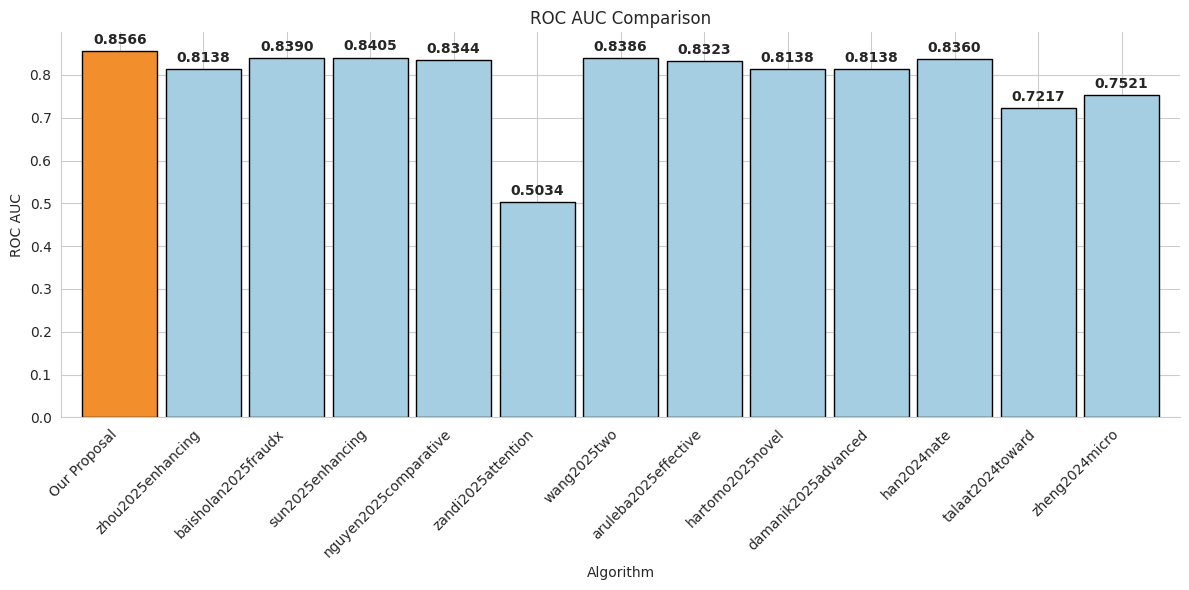
\includegraphics[width=0.95\linewidth]{img/rocauc}
		\caption{Mean ROC~AUC across twelve credit risk datasets. The dashed line indicates the best value achieved by the compared approaches; the dotted line indicates PbCRPE's value.}
		\label{fig:rocauc}
	\end{figure}
	
	\begin{figure}[htbp]
		\centering
		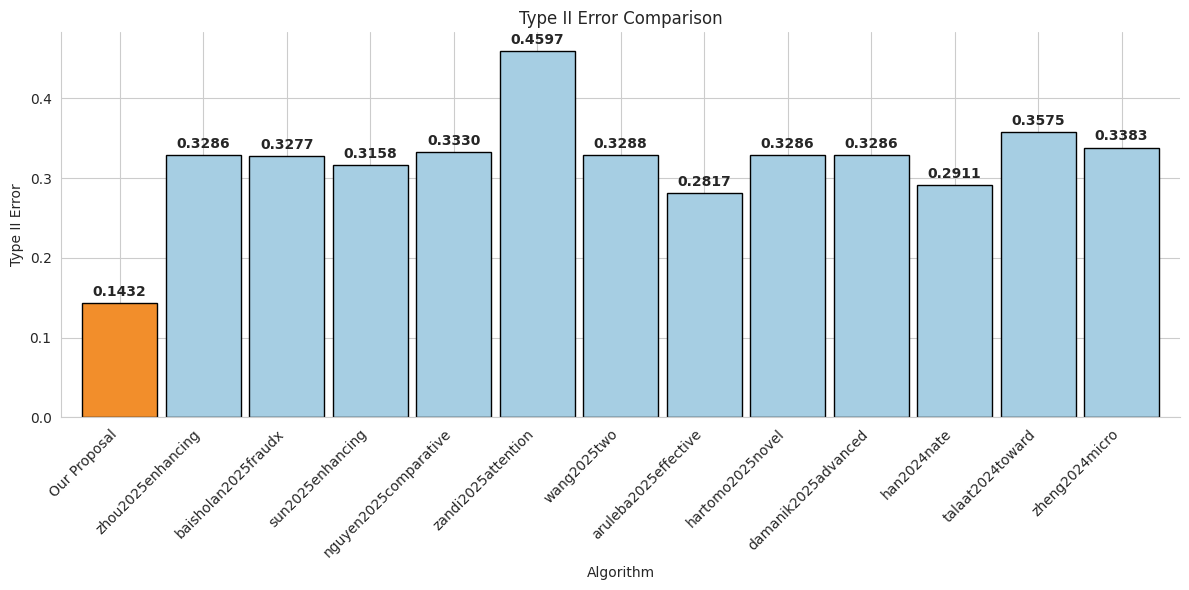
\includegraphics[width=0.95\linewidth]{img/errortipoII}
		\caption{Mean Type~II Error (false negative rate) across twelve credit risk datasets. Lower values indicate better performance. The dashed line indicates the lowest value achieved by the compared approaches; the dotted line indicates PbCRPE's value.}
		\label{fig:type2}
	\end{figure}
	
	Averaged across all twelve datasets, PbCRPE achieves a mean ROC~AUC of \textbf{0.8566} and a Type~II Error of \textbf{0.1432}, outperforming the average values obtained by all state-of-the-art works included in the comparison. A per-dataset analysis confirms that PbCRPE obtains the highest ROC~AUC in several individual datasets and maintains competitive performance across the remaining scenarios. Similarly, PbCRPE achieves lower Type~II Error in multiple datasets, indicating a better ability to identify actual defaulters. The variations observed between ROC~AUC and Type~II Error across some datasets are expected, as these metrics capture different aspects of predictive performance: ROC~AUC reflects overall discrimination capability, while Type~II Error specifically measures the identification of true defaulters. In credit risk prediction, reducing Type~II Error is of primary practical importance, since failing to identify a defaulter may result in direct financial losses for lending institutions, whereas incorrectly classifying a non-defaulter as a defaulter generally represents a missed business opportunity rather than an immediate financial loss.
	
	% ─────────────────────────────────────────────────────────────────────────────
	\subsection{Discussion}
	
	PbCRPE achieves competitive predictive performance compared with the twelve evaluated state-of-the-art approaches while simultaneously providing an explanation for each prediction. This dual capability — prediction and explanation within a single algorithm — represents a structural advantage over post-hoc techniques such as SHAP and LIME, which assign importance scores to individual features independently and do not explicitly represent the joint effect of feature-value combinations. This distinction is particularly relevant in credit risk prediction, where default risk is typically associated with combinations of financial and personal features rather than isolated features~\cite{aruleba2025improved}.\\
	
	The explanations generated by PbCRPE are represented as contrast patterns consisting of conjunctions of $feature\#value$ conditions, providing a rule-based and human-understandable justification for each prediction. For example, in the German credit dataset, a \textit{bad credit risk} prediction for a new instance can be explained by the following contrast pattern:
	\[
	\begin{aligned}
		&\mathit{credit\_history} \neq \texttt{A34} \wedge
		\mathit{amount} < \$7{,}824 \wedge
		\mathit{duration} > 28\,\mathrm{months} \\
		&\wedge\ \mathit{interest\_rate} > 2\% \wedge
		\mathit{num\_loans} \leq 1
	\end{aligned}
	\]
	
	The new instance covered by this contrast pattern is characterized by the following feature values:
	
	\begin{center}
		\small
		\captionof{table}{Example instance covered by the selected contrast pattern.}
		\label{tab:example_instance}
		\begin{tabular}{@{}ll@{}}
			\hline
			\textbf{Attribute} & \textbf{Value} \\
			\hline
			Checking status & No checking account \\
			Duration & 36 months \\
			Credit history & Critical account \\
			Purpose & Radio / Television \\
			Credit amount & \$3,342 \\
			Interest rate & 4\% \\
			Existing loans & 1 \\
			\hline
		\end{tabular}
	\end{center}
	
	The selected contrast pattern represents the conjunction of $feature\#value$ conditions that characterize the new instance and are also satisfied by multiple similar instances within the selected cluster. Therefore, the explanation is not based on isolated feature contributions, but on a combination of conditions associated with the predicted credit risk class. This format is similar to the reasoning style used in traditional credit risk prediction, where decisions are commonly justified through explicit combinations of applicant attributes, facilitating adoption in regulated
	environments that require explainable decisions.\\
	
	The integration of K-modes clustering prior to contrast pattern mining plays a key role in obtaining specific and locally representative patterns. Instead of mining patterns intended to represent all instances of a class, contrast patterns are extracted from groups of similar instances, resulting in more specific conditions associated with local data structures. During the explanation stage, the similarity between a new instance and each cluster is evaluated using the support of the patterns covering the instance, allowing PbCRPE to identify the cluster whose patterns best characterize the new instance. The contrast pattern with the highest support among those covering the new instance is then selected as the explanation. Experimentally, all evaluated instances were covered by at least one contrast pattern mined from a cluster associated with the predicted class, indicating that the proposed clustering and pattern mining strategy achieved complete coverage on the twelve evaluated datasets.\\
	
	Taken together, these results suggest that PbCRPE provides a combination of predictive performance and explainable for credit risk prediction on mixed-type and imbalanced datasets, two characteristics that are common in real-world lending scenarios.
	
	
}